\documentclass[border=1mm]{standalone}

\usepackage[dvipsnames]{xcolor}
\usepackage{tikz}

\begin{document}
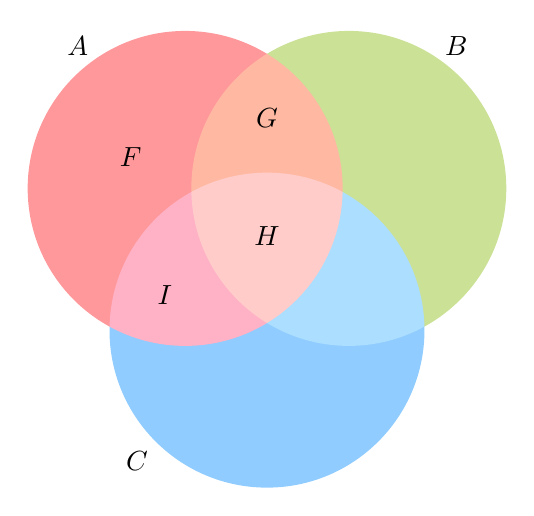
\begin{tikzpicture}
	\definecolor{vennred}{HTML}{ff989b}
	\definecolor{vennblue}{HTML}{90ccff}
	\definecolor{venngreen}{HTML}{cbe196}
	\begin{scope}[blend group = soft light]
		%						\fill[red!30!white!90]   ( 150:1.2) circle (2);
		\fill[vennred]   ( 150:1.2) circle (2);
		%						\fill[blue!30!white!90] (270:1.2) circle (2);
		\fill[vennblue] (270:1.2) circle (2);
		%						\fill[green!30!white!90]  (30:1.2) circle (2);
		\fill[venngreen]  (30:1.2) circle (2);
	\end{scope}
	\node at (135:3.4) {$ A $};
	\node at (45:3.4) {$ B $};
	\node at (240:3.3)	{$ C $};
	\node at ( 150:2)    {$ F $};
	\node at (90:1.5) 	{$ G $};
	\node at (210:1.5) 	{$ I $};
	\node [] {$ H $};
\end{tikzpicture}

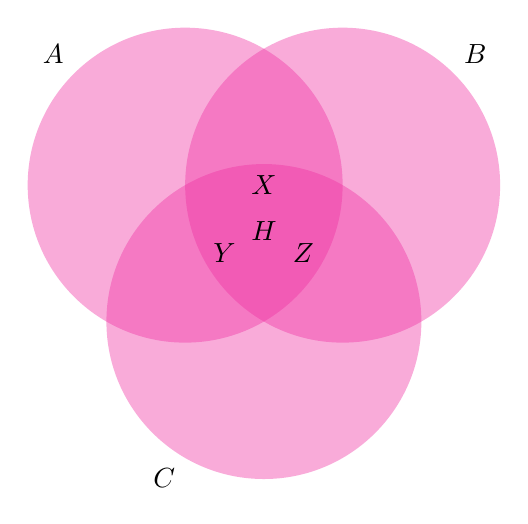
\begin{tikzpicture} [set/.style = {%draw,
		circle,
		minimum size = 4cm,
		fill=Rhodamine,
		opacity = 0.4,
		text opacity = 1}]

	\node (A) [set, label = {135:$A$}] {};
	\node (C) at (300:2cm) [set, label = {240:$ C $}] {};
	\node (B) at (0:2cm) [set, label = {45:$ B $}] {};

	\node at (barycentric cs:A=1,B=1) [] {$X$};
	\node at (barycentric cs:A=1,C=1) [] {$Y$};
	\node at (barycentric cs:B=1,C=1) [] {$Z$};
	\node at (barycentric cs:A=1,B=1,C=1) [] {$H$};

\end{tikzpicture}
\end{document}